%%%%%%%%%%%%%%%%%%%%%%%%%%%%%%%%%%%%%%%%%%%%%%%%%%%%%%%%%%%%%%%%%%%%%%%%%%%%%%%%%%
\begin{frame}[fragile]\frametitle{}
\begin{center}
{\Large Introduction to Statistical Distributions}
\end{center}
\end{frame}


%%%%%%%%%%%%%%%%%%%%%%%%%%%%%%%%%%%%%%%%%%%%%%%%%%%%%%%%%%%%%%%%%%%%%%%%
\begin{frame}[fragile]\frametitle{What is a Statistical Distribution?}

Example
\begin{columns}
    \begin{column}[T]{0.6\linewidth}
	\begin{itemize}
	\item Say, we are measuring height of people and we plotted histogram.
	\item Measurements in the middle are more than at the ends (extreme values).
	\item If we decrease the bin size to very small width, and with lots of observations, we will get a continuous curve approximating the tops.
	\item The curve gives a general sense, so we still can calculate frequencies of the missing observations.
	\end{itemize}

    \end{column}
    \begin{column}[T]{0.4\linewidth}
      \begin{center}
      \includegraphics[width=\linewidth,keepaspectratio]{statq10}
	  
	  \includegraphics[width=\linewidth,keepaspectratio]{statq11}
	  
	  \includegraphics[width=\linewidth,keepaspectratio]{statq12}	  
	  	\end{center}
    \end{column}

  \end{columns}
  
Thats `normal' distribution.

\tiny{(Ref: StatQuest: What is a statistical distribution? - Josh Starmer )}
\end{frame}


%%%%%%%%%%%%%%%%%%%%%%%%%%%%%%%%%%%%%%%%%%%%%%%%%%%%%%%%%%%%%%%%%%%%%%%%
\begin{frame}[fragile]\frametitle{`Normal' or `Gaussian' Distribution}
Also called `Bell Curve'.

\begin{columns}
    \begin{column}[T]{0.6\linewidth}
	\begin{itemize}
	\item More people are in the middle region. 
	\item Thats also a relative probability saying that its more likely to find someone of average height.
	\item Its less likely (low probability) to find someone very tall or very short.
	\item Another example: two normal distributions of the height of male humans when born and as adults.
	\item For babies, almost all of them have similar heights (20 inches), but as adults variations are more.
	\end{itemize}

    \end{column}
    \begin{column}[T]{0.4\linewidth}
      \begin{center}
      \includegraphics[width=\linewidth,keepaspectratio]{statq13}
	  
	  \includegraphics[width=\linewidth,keepaspectratio]{statq14}
	   
	  	\end{center}
    \end{column}

  \end{columns}
  
\tiny{(Ref: StatQuest: What is a statistical distribution? - Josh Starmer )}
\end{frame}


%%%%%%%%%%%%%%%%%%%%%%%%%%%%%%%%%%%%%%%%%%%%%%%%%%%%%%%%%%%%%%%%%%%%%%%%
\begin{frame}[fragile]\frametitle{`Normal' or `Gaussian' Distribution}
      \begin{center}
      \includegraphics[width=0.8\linewidth,keepaspectratio]{statq15}
	  
	  \includegraphics[width=0.8\linewidth,keepaspectratio]{statq16}
    \end{center}
		

\tiny{(Ref: StatQuest: What is a statistical distribution? - Josh Starmer )}
\end{frame}

%%%%%%%%%%%%%%%%%%%%%%%%%%%%%%%%%%%%%%%%%%%%%%%%%%%%%%%%%%%%%%%%%%%%%%%%
\begin{frame}[fragile]\frametitle{Width of the curve is represented by Standard deviation.}

      \begin{center}
  
	   
	  \includegraphics[width=0.8\linewidth,keepaspectratio]{statq17}
	   
      \includegraphics[width=0.8\linewidth,keepaspectratio]{statq18}	   
	  	\end{center}
		

\tiny{(Ref: StatQuest: What is a statistical distribution? - Josh Starmer )}
\end{frame}

%%%%%%%%%%%%%%%%%%%%%%%%%%%%%%%%%%%%%%%%%%%%%%%%%%%%%%%%%%%%%%%%%%%%%%%%
\begin{frame}[fragile]\frametitle{`Normal' or `Gaussian' Distribution}
      \begin{center}

	  
	  \includegraphics[width=0.8\linewidth,keepaspectratio]{statq19}
	   
   
	  \includegraphics[width=0.8\linewidth,keepaspectratio]{statq20}
	   
	  	\end{center}
		

\tiny{(Ref: StatQuest: What is a statistical distribution? - Josh Starmer )}
\end{frame}

%%%%%%%%%%%%%%%%%%%%%%%%%%%%%%%%%%%%%%%%%%%%%%%%%%%%%%%%%%%%%%%%%%%%%%%%
\begin{frame}[fragile]\frametitle{`Normal' or `Gaussian' Distribution}

	\begin{itemize}
	\item Normal Distribution is observed widely in nature, eg heights, weights, incomes, etc
	\item The reason behind this is: The Central Limit Theorem.
	\item Briefly, if you plot averages of samples, they form normal distribution.
	
	\end{itemize}

  
\tiny{(Ref: StatQuest: What is a statistical distribution? - Josh Starmer )}
\end{frame}

%%%%%%%%%%%%%%%%%%%%%%%%%%%%%%%%%%%%%%%%%%%%%%%%%%%%%%%%%%%
\begin{frame}
\frametitle{Mathematically, The normal distribution}

The normal (or Gaussian) distribution is a continuous, symmetric distribution.

The {\bf standard normal distribution}, denoted $N(0,1)$ is a normal
distribution with mean 0 and variance 1.  The normal distribution
$N(\mu, \sigma^2)$ has mean $\mu$ and variance $\sigma^2$.

From the properties of expected values and standard deviations given earlier:

\begin{itemize}

\item If $Z$ is standard normal, then $\mu + \sigma Z$ is
  $N(\mu,\sigma^2$).

\item If $Z$ is $N(\mu, \sigma^2)$, then $(Z-\mu)/\sigma$ is standard
  normal.

\end{itemize}

\end{frame}

%%%%%%%%%%%%%%%%%%%%%%%%%%%%%%%%%%%%%%%%%%%%%%%%%%%%%%%%%%%%%%%%%%%%%%%%
\begin{frame}[fragile]\frametitle{Sampling a Distribution}
\begin{columns}
    \begin{column}[T]{0.6\linewidth}
	\begin{itemize}
	\item If we take one sample from a Normal Distribution, most likely it will be a value near middle.
	\item Once in a while we may get values from ends as well.
	\item Why do you take samples: to explore the statistics.
	\item Rather than measuring all, to explore using only a few values.
	\end{itemize}

    \end{column}
    \begin{column}[T]{0.4\linewidth}
      \begin{center}
      \includegraphics[width=\linewidth,keepaspectratio]{statq21}
	  
	  \includegraphics[width=\linewidth,keepaspectratio]{statq22}
	   
	  	\end{center}
    \end{column}

  \end{columns}
  
\tiny{(Ref: StatQuest: What is a statistical distribution? - Josh Starmer )}
\end{frame}

%%%%%%%%%%%%%%%%%%%%%%%%%%%%%%%%%%%%%%%%%%%%%%%%%%%%%%%%%%%%%%%%%%%%%%%%
\begin{frame}[fragile]\frametitle{Sampling a Distribution}
\begin{columns}
    \begin{column}[T]{0.6\linewidth}
	\begin{itemize}
	\item Tests can be used to see if the samples represent the original population data.
	\item We can measure similarity between two samples as well, by t-test.
	\item Since the original distribution form both is same, should give large p value (meaning both are mostly same)
	\item With just 3 samples for different distributions if p value is small, then increase the sample size.
	\end{itemize}

    \end{column}
    \begin{column}[T]{0.4\linewidth}
      \begin{center}
      \includegraphics[width=\linewidth,keepaspectratio]{statq23}
	  
	  \includegraphics[width=\linewidth,keepaspectratio]{statq24}
	   
	  	\end{center}
    \end{column}

  \end{columns}
  
 Calculating normal probabilities meaning sampling normal distribution.
 
\tiny{(Ref: StatQuest: What is a statistical distribution? - Josh Starmer )}
\end{frame}



%%%%%%%%%%%%%%%%%%%%%%%%%%%%%%%%%%%%%%%%%%%%%%%%%%%%%%%%%%%
\begin{frame}[fragile]
\frametitle{Calculating normal probabilities}

Suppose we have a random variable $T$ which has mean $\mu$ and
variance $\sigma^2$.  If we are willing to assume $T$ is normal, how
can we calculate $P(T>c)$ for some constant $c$?

Normal probability tables are available on the web and in most
statistics software packages.  Often only a table for the standard
normal distribution is available, but this is sufficient, since

\vspace{-0.5cm}

\begin{eqnarray*}
P(T>c) &=& P((T-\mu)/\sigma > (c-\mu)/\sigma)\\ &=& 1 - P(Z \le
(c-\mu)/\sigma).
\end{eqnarray*}

Thus we can look up the value of $(c-\mu)/\sigma$ in a standard normal
probability, table or use a software package, e.g. in R we would use

\begin{lstlisting}
1 - pnorm((c-mu)/s)
\end{lstlisting}

\end{frame}

%%%%%%%%%%%%%%%%%%%%%%%%%%%%%%%%%%%%%%%%%%%%%%%%%%%%%%%%%%%
\begin{frame}
\frametitle{Normal distribution rules of thumb}

\begin{itemize}

\item The normal distribution is symmetric -- around half of a normal
sample lies below the mean and half lies above the mean.

\item Around 68\% of a normal sample lies within one standard
deviation of the mean.  For example, if we have 1000 points from a
normal distribution with mean $10$ and variance $4$, around 680 of the
points will lie between 8 and 12.

\item Around 95\% of a normal sample lies within two standard
  deviations of the mean.  Continuing with the previous example,
  around 950 of the points will lie between 6 and 14.

\item Around 99\% of a normal sample lies within three standard
  deviations of the mean.  Continuing with the previous example,
  around 990 of the points will lie between 4 and 16.

\end{itemize}

\end{frame}



%%%%%%%%%%%%%%%%%%%%%%%%%%%%%%%%%%%%%%%%%%%%%%%%%%%%%%%%%%%%%%%%%%%%%%%%
\begin{frame}[fragile]\frametitle{Normal Distribution}
The classic bell curve-shaped distribution and is completely determined by two parameters: its mean (mu) and its standard deviation	 (sigma).
\begin{center}
\includegraphics[width=0.6\linewidth,keepaspectratio]{normdisteq}
\end{center}
Implement. 

Use \lstinline|math.sqrt| and \lstinline|math.pi| as well as \lstinline|matplotlib.pyplot| for plotting
\begin{lstlisting}
def normal_pdf(x, mu=0, sigma=1):
	:
	return v
\end{lstlisting}
\end{frame}

%%%%%%%%%%%%%%%%%%%%%%%%%%%%%%%%%%%%%%%%%%%%%%%%%%%%%%%%%%%%%%%%%%%%%%%%
\begin{frame}[fragile]\frametitle{Normal Distribution}
Data and plotting routine
\begin{lstlisting}
xs=[x	/10.0 for x in range(-50, 50)]

plt.plot(xs,[normal_pdf(x,sigma=1) for x in xs],'-')
plt.plot(xs,[normal_pdf(x,sigma=2) for x in xs],'--')
plt.plot(xs,[normal_pdf(x,sigma=0.5) for x in xs],':')
plt.plot(xs,[normal_pdf(x,mu=-1) for x in xs],'-')
plt.legend()
plt.title("Normal pdfs")
plt.show()
\end{lstlisting}
\end{frame}

%%%%%%%%%%%%%%%%%%%%%%%%%%%%%%%%%%%%%%%%%%%%%%%%%%%%%%%%%%%%%%%%%%%%%%%%
\begin{frame}[fragile]\frametitle{Normal Distribution}
\begin{lstlisting}
import math
import matplotlib.pyplot as plt
def normal_pdf(x, mu=0, sigma=1):
	sqrt_two_pi = math.sqrt(2*math.pi)
	return	(math.exp(-(x-mu)**2/2/sigma**2) / (sqrt_two_pi* sigma))
\end{lstlisting}
\end{frame}

%%%%%%%%%%%%%%%%%%%%%%%%%%%%%%%%%%%%%%%%%%%%%%%%%%%%%%%%%%%%%%%%%%%%%%%%
\begin{frame}[fragile]\frametitle{Normal Distribution}
\begin{center}
\includegraphics[width=0.8\linewidth,keepaspectratio]{normdistplot}
\end{center}
\end{frame}


%%%%%%%%%%%%%%%%%%%%%%%%%%%%%%%%%%%%%%%%%%%%%%%%%%%%%%%%%%%
\begin{frame}
\frametitle{Log transforms}

Some quantities that vary over several orders of magnitude are best
analyzed on the log scale.

For example, if we observe these values:

$$
14,28,3,60,39,13,1,9,3,55
$$

We can take $\log_2$ to get their approximate values as powers of 2:

$$
3.8, 4.8, 1.6, 5.9, 5.3, 3.7, 0, 3.2, 1.6, 5.8.
$$

It usually doesn't matter what base is used, since we can convert from
one base to another by scaling:

$$
\log_b(x) = \log_a(x) / \log_a(b)
$$

\end{frame}

%%%%%%%%%%%%%%%%%%%%%%%%%%%%%%%%%%%%%%%%%%%%%%%%%%%%%%%%%%%
\begin{frame}
\frametitle{Symmetrizing effect of log transforms}

The log transform symmetrizes right-skewed distributions:

\begin{center}
\begin{tabular}{cc}
\scalebox{0.3}{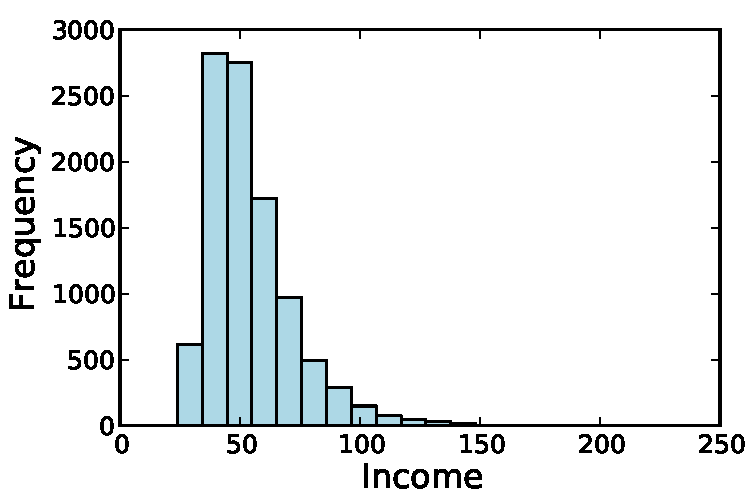
\includegraphics{042-1.pdf}} &
\scalebox{0.3}{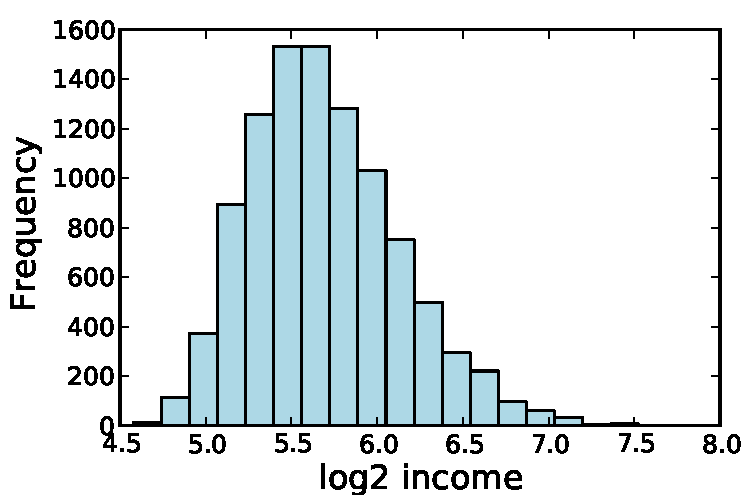
\includegraphics{042-2.pdf}} 
\end{tabular}
\end{center}

It's common to transform data to make it more symmetric, and usually
that's the right thing to do (but don't overdo it...).


\end{frame}

%%%%%%%%%%%%%%%%%%%%%%%%%%%%%%%%%%%%%%%%%%%%%%%%%%%%%%%%%%%
\begin{frame}
\frametitle{Properties of log transforms}

Remember the key properties of logarithms: 

$$\log(ab) = \log(a) + \log(b) \hspace{2cm} \log(a^b) = b\log(a).$$

As a consequence, if we take data $X_1, \ldots, X_n$ and scale it to
get $Z_i = cX_i$, then

$$
\log(Z_1), \ldots, \log(Z_n) = \log(c)+\log(X_1), \ldots, \log(c)+\log(X_n)
$$

Thus changing the units of the original data becomes a shift by
$\log(c)$ units for the log-transformed data.

\end{frame}

%%%%%%%%%%%%%%%%%%%%%%%%%%%%%%%%%%%%%%%%%%%%%%%%%%%%%%%%%%%
\begin{frame}
\frametitle{Mean values and log transforms}

If we observe data $X_1, \ldots, X_n$ and take a log transform to get
$Y_i = \log X_i$, then the mean value of the logged data is:

\begin{eqnarray*}
\bar{Y} &=& n^{-1}\sum_i Y_i\\
       &=& n^{-1}\sum_i \log X_i\\
       &=& n^{-1}\log(X_1 \cdot X_2 \cdots X_n)\\
       &=& \log\left((X_1 \cdot X_2 \cdots X_n)^{1/n}\right).
\end{eqnarray*}

$(X_1 \cdot X_2 \cdots X_n)^{1/n}$ is called the {\bf geometric mean}
of the $X_i$, so we see that the usual (arithmetic) mean of the log
transformed data is the log of the geometric mean of the untransformed
data.

\end{frame}


\begin{frame}
\frametitle{Log transforms}

We generally take the log of positive data that is substantially right
skewed.  If the data are roughly symmetrically distributed, there is
no need to take a log transform, and you cannot take a log transform
if any of the data values are less than or equal to zero.

\textcolor{blue}{\bf Examples:} We generally would log-transform
income but not age.


\end{frame}



%%%%%%%%%%%%%%%%%%%%%%%%%%%%%%%%%%%%%%%%%%%%%%%%%%%%%%%%%%%
\begin{frame}
\frametitle{Standardizing the sample mean}

Suppose we have an id sample of $n$ observations from a population
with mean $\mu$ and variance $\sigma^2$.

We know that $\bar{X}$ has mean $\mu$ and variance $\sigma^2/n$ (so
the standard deviation is $\sigma/\sqrt{n}$).  

The standardized sample mean is

$$
\frac{\bar{X}-\mu}{\sigma/\sqrt{n}} = \sqrt{n}\frac{\bar{X}-\mu}{\sigma}.
$$

\end{frame}


\begin{frame}
\frametitle{Example calculation with the normal distribution}

Suppose we have a sample $X_1, \ldots, X_{20}$ from a normal
population with mean zero.  We are told that the probability that
$|\bar{X}|$ is greater than 1 is 0.2.  What is the standard deviation
of the $X_i$?

Using the fact that the normal distribution is symmetric,

\begin{eqnarray*}
0.2 &=& P(|\bar{X}| > 1)\\ &=& P(\bar{X}>1) + P(\bar{X}<-1)\\ &=&
2P(\bar{X}>1)\\ &=&
2P(\sqrt{20}\bar{X}/\sigma>\sqrt{20}/\sigma)\\ &=& 2P(Z >
\sqrt{20}/\sigma).
\end{eqnarray*}

So $P(Z > \sqrt{20}/\sigma) = 0.1$.  Now if we look at a table of the
normal distribution, we see that the probability of a standard normal
value being bigger than 1.28 is 0.1, so $\sqrt{20}/\sigma = 1.28$, and
$\sigma = \sqrt{20}/1.28 \approx 3.49$.

\end{frame}


\begin{frame}
\frametitle{Exercises}

\begin{enumerate}

\item Suppose we observe a sample of 100 values from a normal
 population with mean 100 and standard deviation 10.  Around how many
 of the values will be greater than 110?

\item Suppose we observe a sample of 150 values from a normal
 population with mean 80 and standard deviation 12.  Write an R
 expression that will give the approximate number of values between
 75 and 85.

\item Suppose we observe a sample of 200 values from a normal
 distribution with mean zero.  Around 20 of the values that we
 observe are greater than 50.  Approximately what is the standard
 deviation of the population we are sampling from?

\end{enumerate}

\end{frame}
